\chapter{Team Coordination}
\label{Coordination}

In this chapter, we are going to present the most important, exciting, and time-consuming part of this thesis. Up to this chapter, we have discussed all skills that agents need in order to be functional in the soccer field. With these functionalities agents are able to locate themselves in the field, communicate with each other, and execute actions combining movements through the motion controller. However, agents miss a thinking process with which they will be able to decide what action they should take for the global benefit of the team. In real human soccer, this will correspond to players with excellent individual skills for a soccer match, but no reasoning ability to choose what is best to do at each time. Therefore, it is crucial to come up with a high-level process which will coordinate all these skills, motions, communication ability, and actions yielding as a result a complete behavior for each agent within the frame of a global team strategy. As behavior, we define the process in which an agent takes as input arguments its beliefs and decides what to do as an output. 

\section{Coordination Protocol}

In our approach, instead of each agent deciding its own behavior, players depend on a centralized process, called team coordination, which implicitly determines individual behaviors for each agent.  The team coordination algorithm is responsible for gathering messages from all agents and producing appropriate actions for all agents towards achieving a common goal. We choose one player (by default, the goalkeeper) to act as the central coordinator, that is the one who is going to execute this team coordination procedure on behalf of the entire team. This means that all players communicate their beliefs to the goalkeeper, the goalkeeper executes the team coordination procedure for the entire team, and finally the goalkeeper sends back to the players the actions they are required to take.


\begin{figure}[t!]
\centering
  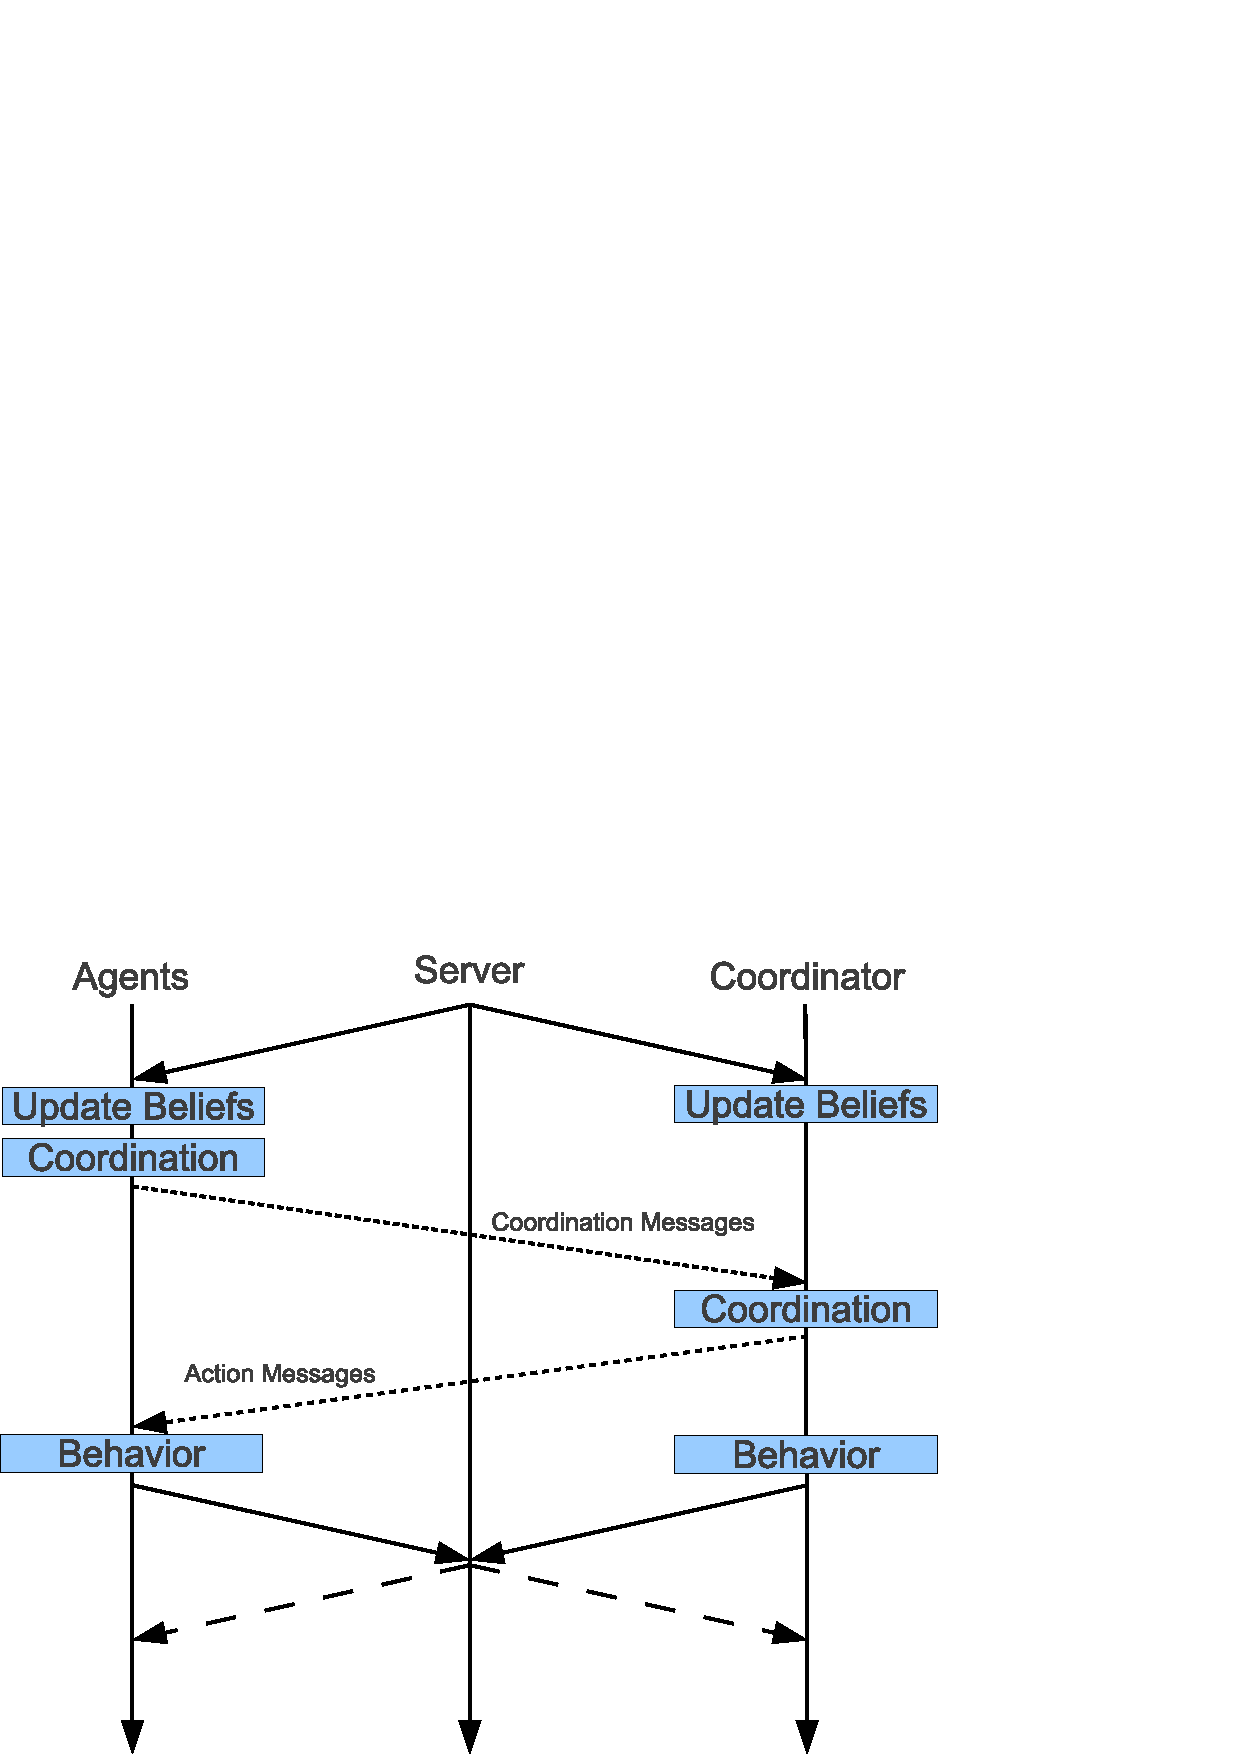
\includegraphics[width=0.6\textwidth]{Chapter4/figures/CoordinationCycle.pdf}
  \caption{The Coordination Protocol.} 
  \label{fig:CoordinationCycle}
\end{figure}


Figure~\ref{fig:CoordinationCycle} shows the entire coordination protocol (which may last several simulation cycles). All players initially update their beliefs. The coordinator (goalkeeper) waits for messages from all other players. Once these messages are gathered at the coordinator, the coordination procedure is executed and the resulting actions for each player are communicated back to the players. At this point all players execute their actions, in essence realizing their behavior. We selected the goalkeeper to act as coordinator, because its role is quite distinct and independent from the other players and therefore it can afford to dedicate more computational resources to the team coordination algorithm compared to the other players. 

The team coordination procedure executed only by the coordinator after all messages have been received is split in several phases:
\begin{description}
%\item[Gather Coordination Messages] The coordinator waits for all players to submit their local beliefs about the world state. This phase is completed as soon as all messages have been received. 
\item[Update Coordination Beliefs] The local world state beliefs from the other players are combined in order to update the global belief about the world state (global ball location, distances of all players from the global ball location, locations of all players). 
\item[Split Players in Subsets] Field players are split into non-overlapping subsets according to their significance in the current game state. These subsets are:
\begin{itemize}
\item \textit{Goalkeeper}: one player, the goalkeeper
\item \textit{Inactive}: players fallen on the ground or players with lost self-location
\item \textit{Active}: three players, the ones closest to the ball
\item \textit{Support}: all remaining players
\end{itemize}
\item[Determine Active Positions] Several candidate positions are determined for the active players.
\item[Coordinate Active Players] The active player closest to the ball is assigned to go to the ball and the best pair of candidate positions is selected for the remaining active players according to a cost function.
\item[Generate Team Formation] A formation is generated for the entire team (excluding the goalkeeper) depending on the current position of the ball in the soccer field.
\item[Assign Team Roles] All team players, except the goalkeeper, are assigned roles taking into account the desired  formation of the team and their current position.
\item[Determine Support Positions]  Candidate positions are determined for the support players. These are determined by the desired team formation, after excluding the roles assumed by the active players and a number of least-significant roles equal to the number of inactive players. 
\item[Coordinate Support Players] The best mapping between support players and support positions according to a cost function is computed.
\end{description}
Algorithm~\ref{CoordinationAlgorithm} describes the entire coordination procedure, which currently lasts six simulation cycles. In each simulation cycle, some, but not all, of the above phases are executed. This choice was dictated by the time limitation of the agent think cycle; with this choice, each group of phases fits within a single simulation cycle causing no delays and enabling real-time operation. 

\begin{algorithm}[ht!]
\caption{Coordination Protocol }
\label{CoordinationAlgorithm}
\begin{algorithmic}[1]
\begin{small}
\STATE {\bf Input: }$Coordination Messages = \lbrace M_{1},M_{2},...,M_{N-1} \rbrace, N = Number Of Players $
\STATE {\bf Output: }$Actions = \lbrace A_{1},A_{2},...,A_{N-1} \rbrace$
\STATE
\IF {$ CoordinationCycle = 1$ }
\STATE $B \leftarrow Update Beliefs(Coordination Messages) $
\STATE $CoordinationCycle = CoordinationCycle + 1$
\ELSIF {$ CoordinationCycle = 2$ }
\STATE $S \leftarrow Coordination Splitter(B) $
\STATE $CoordinationCycle = CoordinationCycle + 1$
\ELSIF {$ CoordinationCycle = 3$ } 
\STATE $P_{active} \leftarrow Active Positions(B,S) $
\STATE $CoordinationCycle = CoordinationCycle + 1$
\ELSIF {$ CoordinationCycle = 4$ }
\STATE $A_{active} \leftarrow Active Coordination(P_{active},S,B) $
\STATE $CoordinationCycle = CoordinationCycle + 1$
\ELSIF {$ CoordinationCycle = 5$ }
\STATE $ F \leftarrow TeamFormation(B) $
\STATE $ R \leftarrow Role Assignment(A_{active},B,F) $
\STATE $ P_{support} \leftarrow Support Positions(R,F,S) $
\STATE $CoordinationCycle = CoordinationCycle + 1$
\ELSIF {$ CoordinationCycle = 6$ }
\STATE $A_{support} \leftarrow Support Coordination(P_{support},S,B,R,F,A_{active}) $
\STATE $Actions = A_{active} \cup A_{support} \cup A_{inactive}$
\STATE $CoordinationCycle = 0$
\ENDIF
\end{small}
\end{algorithmic}
\end{algorithm}


\section{Coordination and Communication}
Coordination is accomplished through communication. We use the common communication channel through the simulation server in order to provide the messaging between players involved in the coordination process. For this reason, communication plays a major role in our approach. The general idea of this communication process among players is that the coordinator (goalkeeper) needs to know all agents' beliefs about the world state before proceed with the execution of the coordination protocol. Furthermore, communication is needed to send the outcome of coordination from the coordinator to all players. 

There are several types of messages, each one of them having different functionality and serving a specific purpose. The arguments of each message are preceded by a single-letter identifier indicating the type of the message. The message types used in our coordination protocol are:
\begin{description}
\item[Init Message] This type of message declares the presence of each agent in the simulation environment. All players, other than the coordinator, must send this message to the coordinator before the coordination protocol begins.
\begin{description}
  \item[{\bf Message format:}] 
  \texttt{i,<Agent Uniform Number> }
\end{description}

\item[Start Message] This type of message is sent only by the coordinator; it declares that all agents are now initialized and ready to begin the coordination process. Each agent receiving this message should immediately start sending coordination messages.

\begin{description}
  \item[{\bf Message format:}] 
  \texttt{s,<Coordinator Uniform Number>}
\end{description}

\item[Coordination Message] This is the most important type of message. It includes information about each agent's beliefs. There are four subtypes of this message depending on  the current beliefs of the agent:
\begin{description}

\item[Type C] The agent has complete awareness of the ball and self location; the message includes the uniform number, the self position, and the ball position.

\begin{description}
  \item[{\bf Message format:}]
  \texttt{c,<Agent Uniform Number>,<Agent X>,<Agent Y>,\\<Ball X>,<Ball Y>}
\end{description}

\item[Type L] The agent has complete awareness only of his own position in the field; the ball is not currently within the field of view and, even though there may be a filtered belief about the ball location, it is better to avoid sending possibly faulty information. The message includes only the uniform number and the self position.

\begin{description}
  \item[{\bf Message format:}]
  \texttt{l,<Agent Uniform Number>,<Agent X>,<Agent Y>}
\end{description}

\item[Type B] The agent has complete awareness of the ball's location, only with respect to itself. The message includes the uniform number, the distance of the ball and the horizontal angle of the ball relative to its own body angle.

\begin{description}
  \item[{\bf Message format:}]
\texttt{b,<Agent Uniform Number>,<Ball Distance>,<Ball Angle>}
\end{description}

\item[Type X] The agent has complete unawareness of the ball and self location or has fallen on the ground. The message includes only the uniform number. These agents join the inactive subset.

\begin{description}
 \item[{\bf Message format:}]
 \texttt{x,<Agent Uniform Number>}
\end{description}

\end{description}
\item[End Message]
This type of message asks the players, other than the coordinator, to stop sending coordination messages. At this point, the coordinator is ready to execute the coordination procedure and calculate actions for all players.
\begin{description}
  \item[{\bf Message format:}] 
  \texttt{e,<Coordinator Uniform Number>}
\end{description}
\item[Action Message]
This type of message is sent only by the administrator; it declares which action each agent has been assigned by the coordination process. These messages are sent at the end of the coordination procedure, when actions for all players have been computed. The message includes the uniform number of the recipient agent, the action identifier, and the possible action parameters. 
\begin{description}
  \item[{\bf Message format:}]
  \texttt{a,<Agent Uniform Number>,<Action ID>,<Action Parameters>}
\end{description}

\end{description}

\begin{figure}[t!]
\centering
  \includegraphics[width=0.8\textwidth]{Chapter4/figures/CoordComm.pdf}
  \caption{Communication Process in Coordination.} 
  \label{fig:coordinationprocess}
\end{figure}

Figure~\ref{fig:coordinationprocess} presents the messaging procedure between the agents in order to coordinate their actions. First, agents have to initialize their presence in the field with ``init'' messages. The coordinator saves these messages and, when all other players have initialized themselves, broadcasts a ``start'' message. This message means that all players are now ready to start the coordination process. In this phase, all players, other than the coordinator, send their ``coordination'' messages to the coordinator. When the coordinator gathers these messages from all players, it broadcasts an ``end'' message to make them stop sending unnecessary ``coordination'' messages. The next phase of this process is the execution of the coordination protocol which lasts six simulation cycles, approximately 120ms. When it finishes, the coordinator broadcasts the resulting actions to each one of the other players using individual ``action'' messages. The receiving agents execute the commanded actions, until a new ``action'' message arrives. While action execution is ongoing, after a timeout period defined by the user (currently set at 20 simulation cycles), the same coordination process is repeated, excluding the initialization phase.


\section{Coordination Beliefs}

In the previous section we presented how players exchange messages with the coordinator. In this section we are going to discuss how the coordinator fuses the individual beliefs received by the other agents into a single global belief. This step is of major importance in any multi-agent system. Having multiple observations of the same world could potentially be a problem. The coordinator has to combine these observations without knowing which one of them is faulty or correct in order to obtain a global realistic representation of the world. Knowledge of the ball and agents' positions is sufficient to execute the coordination algorithm without making guesses.

The global ball position is computed taking into account only the information communicated by the agents using ``type C'' coordination messages. Furthermore, information of the coordinator is taken into account, if the coordinator also has sufficient knowledge about the ball and self location. Apparently, the maximum number of ball observations at any time is the number of all agents, when all of them have sufficient knowledge about the ball and self location.
\begin{figure}[t!]
\centering
  \includegraphics[width=0.8\textwidth]{Chapter4/figures/Ball.pdf}
  \caption{Global Ball Position Estimation from Multiple Ball Observations.} 
  \label{fig:Ball}
\end{figure}
As shown in Figure~\ref{fig:Ball}, different ball observations can differ from each other. In our approach, we use a simple algorithm to estimate the global ball position with accuracy. A threshold is defined (by default, 1 meter) in order to split the observations in subsets. Each subset is assigned a weight equal to the number of observations it contains. Additionally, each subset is represented by the average of the observations it contains. The first incoming observation defines the first subset with weight $1$. For each subsequent incoming observation, we check its distance against all representatives of all existing subsets. If the minimum of these distances is below the threshold, then this new observation is assigned to the subset that gave this minimum distance, updating at the same time the weight and the representative of that subset. Otherwise, the new observation gives rise to a new subset with a single member. 

Figure~\ref{fig:Ball} shows the resulting four subsets for a given set of nine observations. The set with the most observations included is naturally assigned the biggest weight. Consequently, we have to compute our belief about the global ball position.
++++++++++++++++++++++++++++++++++++++++++++++



Given a total number of $N$ observations $o_j$ split into $m$ observation subsets $s_i$, the final ball belief is computed as:
\begin{align*}
{\bf Global Ball Belief} = \sum_{i=1}^m \frac {|s_i|^2} {\sum_{k=1}^m |s_k|^2} \sum_{o_{ij} \in s_i} \cfrac{o_{ij}}{|s_i|}
\end{align*}


The next step towards forming the global beliefs is to determine each agent's position and its distance from the estimated global ball position. Players who have sent a ``Type C'' or ``Type L'' coordination message have already communicated their exact position in the field; their distance from the ball is simply calculated as the distance between the estimated global ball position and the players' position. Players who have sent a ``Type B'' coordination message don't know their exact position in the field, but this can be inferred using the estimated global ball position and the information they submitted about the distance and angle of the ball observation with respect to themselves; their distance from the ball is simply the one they reported. Finally, for players who have sent a ``Type X'' coordination message, we assume an infinite distance to distinguish them from all other players; their position in the field cannot be inferred. 


\section{Subsets in Coordination Process}
The existence of multiple agents makes coordination a complex and computationally expensive problem to be solved by a single agent. In our case, the coordinator (goalkeeper) would have to solve this huge problem for a total of nine players or eleven players, depending on the server's version).
Instead of trying to solve the coordination problem at one level, a simple approach is to first decompose the problem into smaller coordination problems and then solve each one of them. To this end, we split the players into small subsets in which coordination can be achieved quickly to meet real-time requirements. In our approach, there are four such subsets:

\begin{description}
\item[Active subset] Active subset consists of three agents and it is the most important set of agents in the coordination. Agents who constitute this subset have the responsibility of making worthy actions for their team. Moreover, having to compute optimized actions for three players is not too complex for such an important group. 

\item[Inactive subset] Inactive subset consists of agents who have sent ``Type X'' messages. It is the less important set of agents in the coordination procedure. Agents who constitute this subset assigned the same action, to find their positions in the field. Finding their positions will be resulted to be inserted either in the active or in the support subset in the next coordination cycle.

\item[Support subset] Support subset consists of agents who are neither in the active subset nor in the inactive one. Coordinate actions for these agents is the most time consuming and expensive part of the coordination algorithm.

\item[Goalkeeper] We can realize that goalkeeper subsets includes only one agent. The player with the uniform number one is selected to be this agent which is responsible for guarding our goal. Goalkeeper is also the administrator of the coordination process. His independent and individual behavior will be explained in the end of this Chapter, in Section~\ref{GoalKeeper}.
\end{description}

\begin{figure}[t!]
\centering
  \includegraphics[width=0.8\textwidth]{Chapter4/figures/Splitter.pdf}
  \caption{Coordination Splitter.} 
  \label{fig:Splitter}
\end{figure}

\section{Coordination Splitter}
In this section we are going to discuss how the above three groups are generated by coordination splitter. An array full of team's agents is sorted according to the distance each agent has from the ball. We assign to the active subset the agents in the three first positions of the sorted array.
Other agents with distance less than infinity join the support subset.
Recall that we assume $\infty$ distance from ball for the agents who have no knowledge for their position and have not the ball into the field of their view.
In Figure~\ref{fig:Splitter} is presented an example of the coordination splitter's process. Assuming that all agents have complete awareness of their position, we could realize that the agents in the red distance's threshold will join the active subset. The other six agents who have farther distances from ball will join the support subset. Moreover a possible existence of one or more agents which have unawareness about their world state, should lead them joining the inactive subset.

\begin{figure}[t!]
\centering
  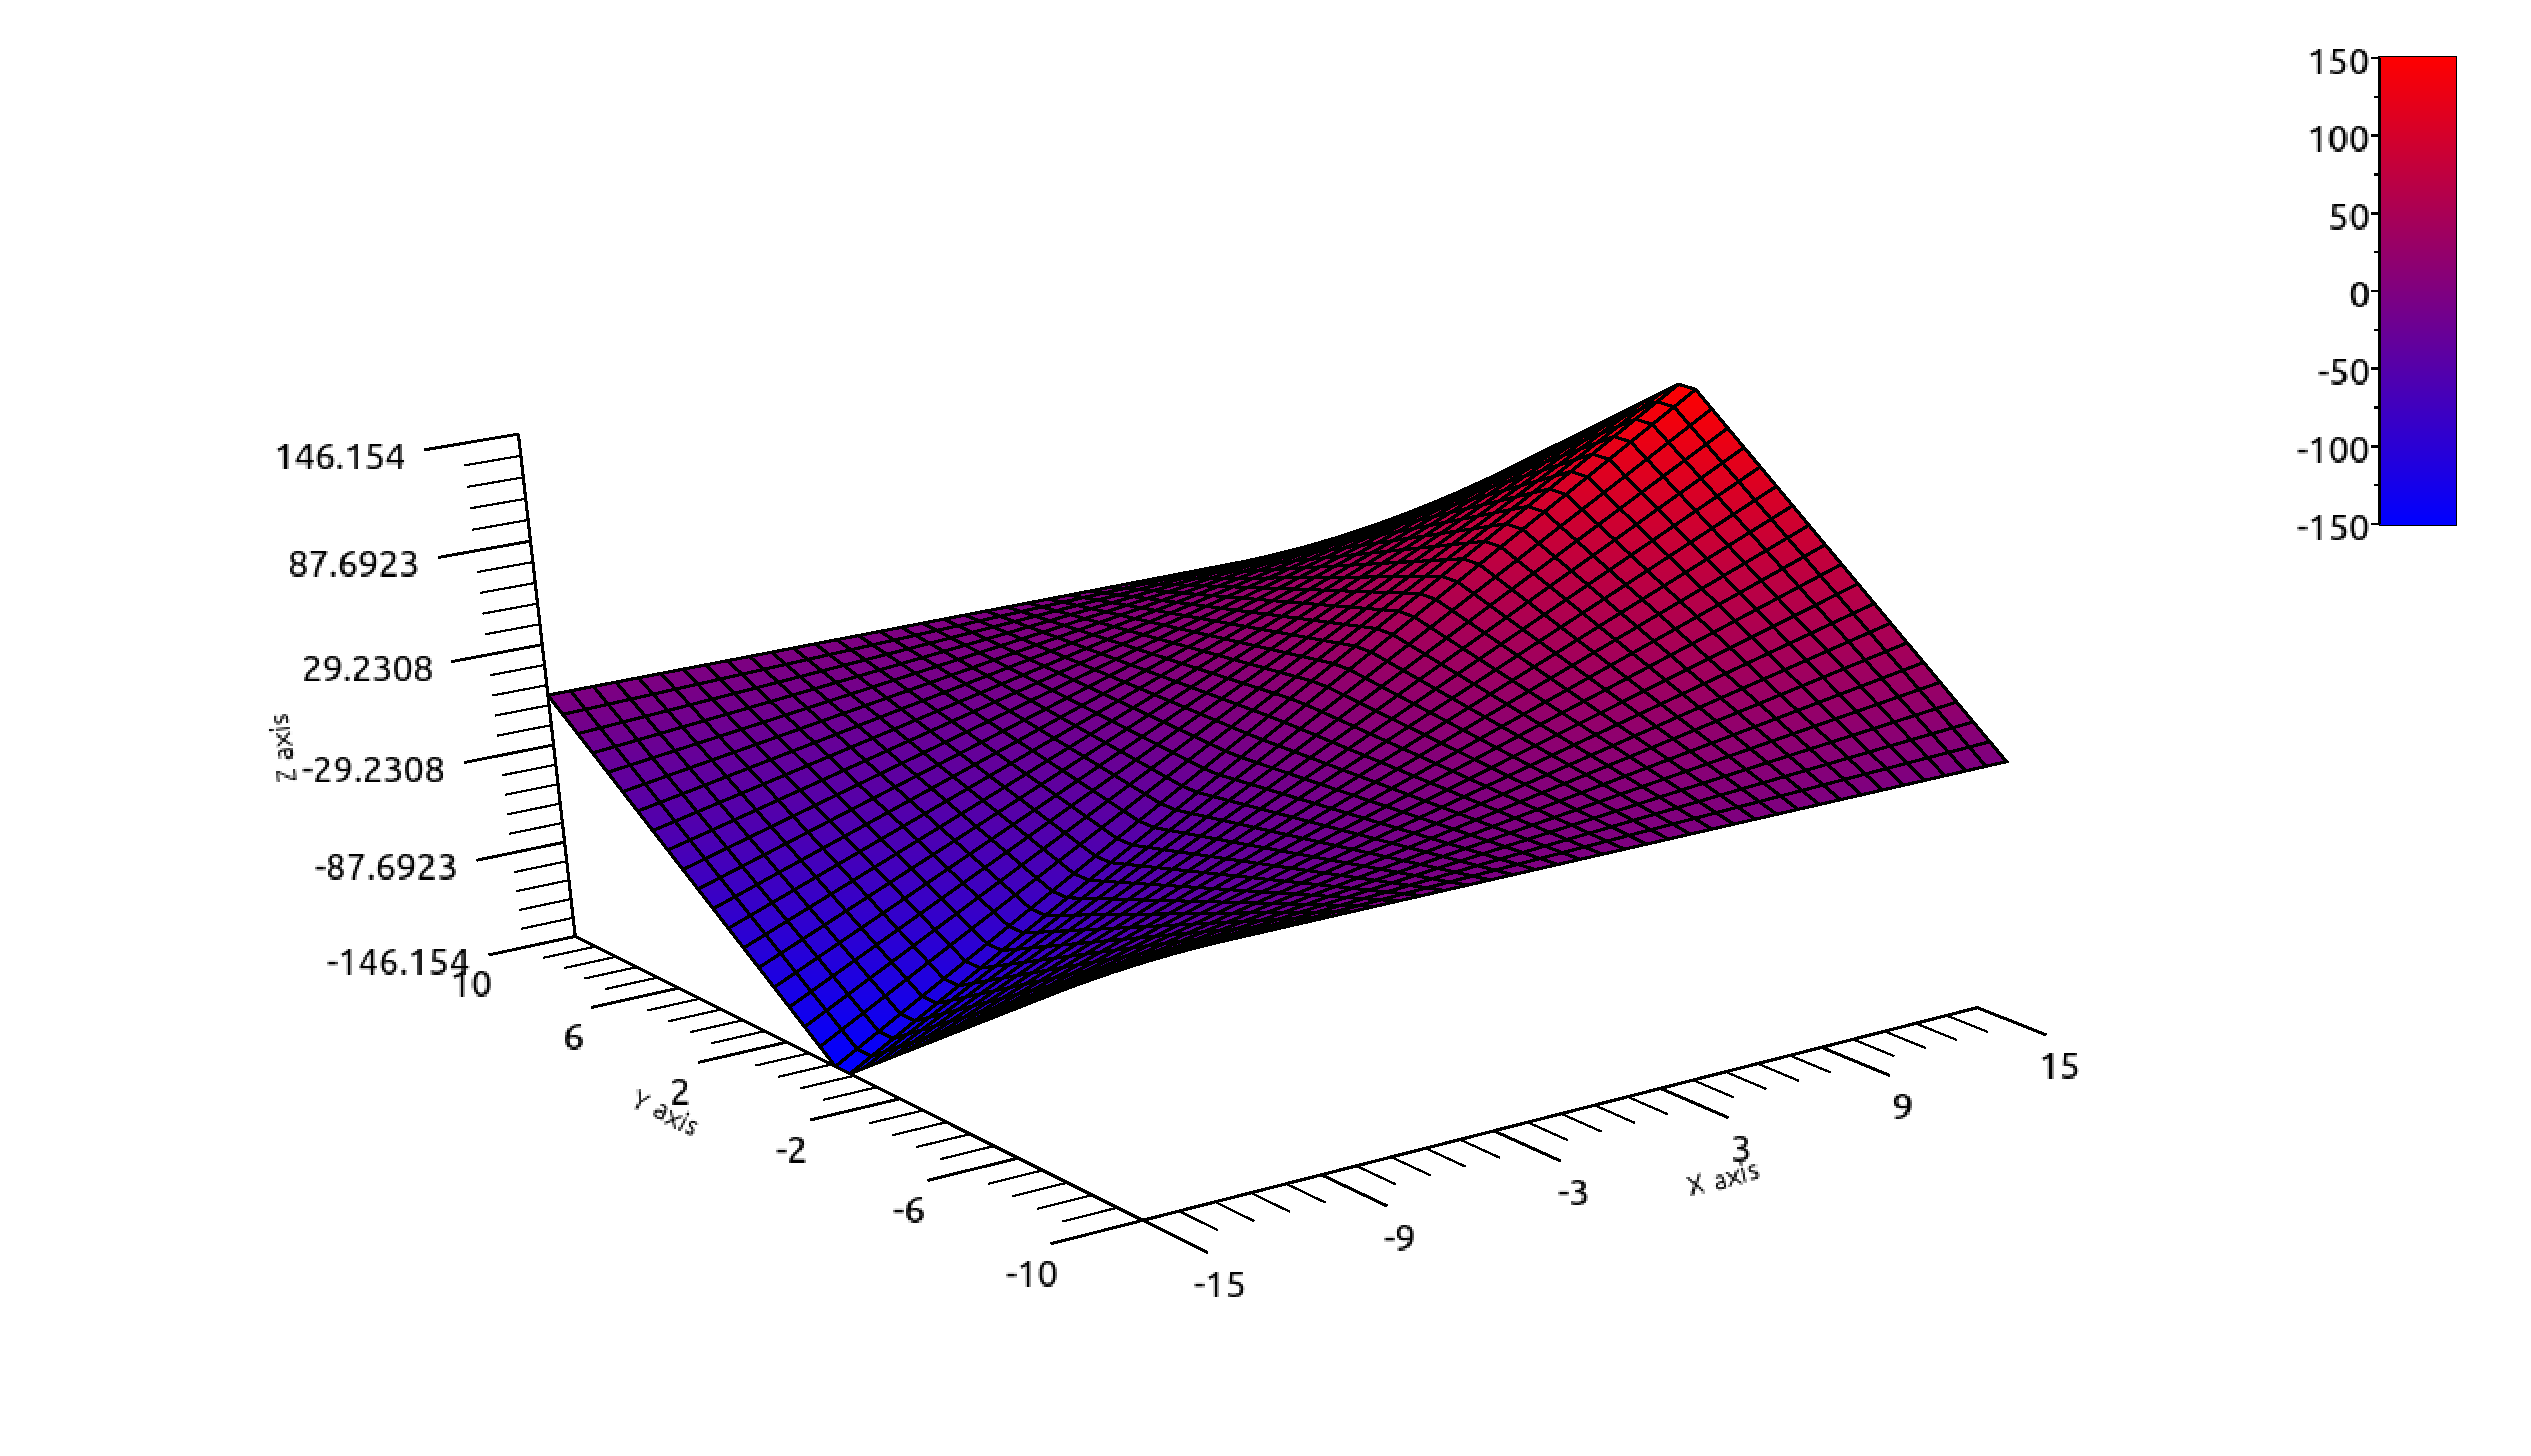
\includegraphics[width=\textwidth]{Chapter4/figures/Graph1.pdf}
  \caption{Soccer Field Value.} 
  \label{fig:SoccerValue}
\end{figure}



\section{Soccer Field Value}
\label{FieldValue}

In order to proceed our discussion about coordination process, we have to demonstrate a simple but functional way to give a value in every spot of the soccer field. Figure~\ref{fig:SoccerValue} presents this evaluation for every spot into the soccer field. The main idea is that as ball heading towards the opponent goal, this value is becoming higher. In contrast, as ball heading towards our goal, this value is becoming lower. We can realize that a big spot value means more chances to score a goal, and a minimum spot value implies a dangerous game situation. This procedure will prove to be useful in the next steps of coordination process.


\begin{figure}[t!]
\centering
  \includegraphics[width=7cm]{Chapter4/figures/ActivePositions2.png}
  \caption{Active positions before elimination.} 
  \label{fig:ActivePositions2}
\end{figure}

\section{Active-Positions Computation}
Until now, we have updated the coordination beliefs and we have split agents into subsets. in this phase of the coordination process, we have to compute adequate and worthy positions for the active subset. We distinguish two cases, in the first case, ball is located in our field's half. In this case we have to find worthy positions which have a defensive approach. On the other hand, if ball is located in the other field's half we have to find positions which have an attacking approach. In both cases we create an array of equidistant coordinates which are located in a radius which is determined by the ball's location and they are not out of soccer field's limits. Figure~\ref{fig:ActivePositions2} shows how these positions are shown in the soccer field through roboviz monitor. 
From these set of coordinates we choose the best according to their values. As we saw in the previous section each coordinate of the field has a utility value. Consequently, we will try to choose a number of coordinates which summarize in a max value in an attacking approach or in a min value in a defensive approach, being careful not to overcome a max number of coordinates which is nine. This will help us later keeping iterations below a maximum number. Figure~\ref{fig:ActivePositions3} shows how active positions are shown in the soccer field through roboviz monitor after elimination. 


\begin{figure}[t!]
\centering
  \includegraphics[width=7cm]{Chapter4/figures/Active3.png}
  \caption{Active positions after elimination.} 
  \label{fig:ActivePositions3}
\end{figure}


\section{Active-Subset Coordination}
Once we have find worthy positions for the active players it is time to find the player who is more adequate than others to become the on ball player. Moreover, we should assign each of the rest two players into an active position. This is called mapping function and will have a significant role in the next coordination's phases. 
\subsection{Player on Ball}
An agent from the active subset has to be selected in order to be sent an action which is related to the ball. We have to find the agent who has minimum value according to two parameters:
\begin{enumerate}
\item \textbf{Distance from ball} $d_{i}$, ball's distance from each agent in the subset. 
\item \textbf{Angle towards goal} $\vartheta_{i}$, this angle is the sum of  the angle between agent's body and the ball and the angle between ball and the opponent's goal.
\end{enumerate}
Given an active subset:

\begin{align*}\
{\bf ActiveSubset} &= \lbrace Agent_{1},Agent_{2},Agent_{3} \rbrace  \\
{\bf Value_{i}} &= d_{i} + a \ast \vartheta_{i}, a\in\mathbb{R} \\
{\bf OnBallPlayer} &= \arg\min_{i}(Value_{i})
\end{align*}
Additionally, we give to the agent who had been assigned an action towards the ball in the previous coordination cycle a small advantage over the others to be again the on ball player. We do this due to the fact that there is a possibility of continuous changes in the on ball player in cases in which two agents have approximately same distances and angles from the ball.



\subsection{Active-Subset Best Mapping}
Next in the active coordination phase, we have to assign positions for the other two agents who have left in the active subset. Algorithm~\ref{ActiveMapping} shows how we can find the optimized mapping. In a greedy approach, we calculate the cost of every possible mapping. In addition, in every mapping we take into account the on ball agent's mapping $(OnBallPlayer \rightarrow Ball)$, which will be helpful in order to find possible collisions between the on ball agent and the active ones.
\begin{algorithm}[ht!]
\caption{Active-Subset Best Mapping}
\label{ActiveMapping}
\begin{algorithmic}[1]
\STATE {\bf Input: }$ActivePlayers = ActiveSubset - Agent_{OnBall} $
\STATE {\bf Input: }$Activepositions = \lbrace P_{1},P_{2},...,P_{N} \rbrace, N\leq 9 $
\STATE {\bf Output: }Optimized Active Mapping
\STATE $OptimActiveMap = \varnothing $
\STATE $S = {{N}\choose{2}}$
\FOR{{\bf each} s in S}
\STATE $ActiveMap = RoleMap[s] \cup (OnBallPlayer \rightarrow Ball)$
\STATE $OptimActiveRoleMap = mincost(ActiveMap,OptimActiveMap)$
\ENDFOR
\end{algorithmic}
\end{algorithm}
We can realize that even we are using a brute force method the number of possible mapping remains able to be computed in real-time. Assuming maximum number of active positions in our case nine, the possible mappings are: ${{9}\choose{2}} = 72$ mappings.


\begin{figure}[t!]
\centering
  \includegraphics[width=0.8\textwidth]{Chapter4/figures/Formation9_0.pdf}
  \caption{Formation Role Positions for 9 vs 9.} 
  \label{fig:Formation9_0}
\end{figure}


\section{Team Formation}
Team formation itself is not a main contribution of this thesis but serves to set up the role assignment function and the coordination of the support subset. In general, team's formation is determined by the ball's position into the field. The formation is broken up into three groups including all players of the team except from goalkeeper. This section presents the team's formation used in our approach for both 0.6.5 and 0.6.6 \textit{rcssserver3d} versions.
\subsection{9-Players Server Version (0.6.5)}
\textbf{Attacking} group which consists of three positions:
\begin{description}
\item[Fc] \textit{Forward center}
\item[Fl] \textit{Forward left}
\item[Fr] \textit{Forward right}
\end{description}
\textbf{Defensive} group which consists of three positions:
\begin{description}
\item[Dc] \textit{Defender center}
\item[Dr] \textit{Defender right }
\item[Dl] \textit{Defender left}
\end{description}
Finally, \textbf{midfield} group which consists of two positions:
\begin{description}
\item[Ml] \textit{Midfielder left}
\item[Mr] \textit{Midfielder right}
\end{description}
As an example, Figure~\ref{fig:Formation9_0} shows how the different role positions of the formation are depicted into the soccer pitch. In general attackers are responsible to be assigned positions near to ball when ball is on the opponents' half of the field. Then, the forward center  is given a position close to the ball and the other two forwards are given positions on either side of the ball in an angle and a distance offset which are determined and dynamically changed according to the ball's exact coordinate. If ball is located in our half, then forwards are given positions which are in the middle of the field. 

On the other hand, defenders are mainly positioned to guard our goal. To determine their position on the field a straight line is computed between our team's goal and the ball. Central defender is given a position placed on this line and its distance from our goal is proportional to the ball's position. The other two defenders' positions are located on either side of the defender center. 

Midfielders' positions are determined by the ball's position as well. For an attacking phase, in which ball is located to the opponents' half of the pitch, midfielders are given position near to the forwards in order to support their attack. In the opposite situation, they are given position in front of our defense line to help defenders. 

Finally, goalkeeper positions himself independently to always be in the best position to stop a shot towards our goal. In some cases, when ball is located near to the field's edges formation positions are adjusted not exceed its limits.

\begin{figure}[t!]
\centering
  \includegraphics[width=0.8\textwidth]{Chapter4/figures/Formation11_0.pdf}
  \caption{Formation Role Positions for 11 vs 11.} 
  \label{fig:Formation11_0}
\end{figure}



\subsection{11-Players Server Version (0.6.6)}
\textbf{Attacking} group which consists of four positions:
\begin{description}
\item[Fc] \textit{Forward center}
\item[Fl] \textit{Forward left}
\item[Fr] \textit{Forward right}
\item[Sf] \textit{Support Forward}
\end{description}
\textbf{Defensive} group which consists of three positions:
\begin{description}
\item[Dc] \textit{Defender center}
\item[Dr] \textit{Defender right }
\item[Dl] \textit{Defender left}
\end{description}
Finally, \textbf{midfield} group which consists of two positions:
\begin{description}
\item[Mc] \textit{Midfielder center}
\item[Ml] \textit{Midfielder left}
\item[Mr] \textit{Midfielder right}
\end{description}



Figure~\ref{fig:Formation11_0} depicts how the different role positions of the formation shown in the soccer pitch for the newest server version in which team consists of eleven players. Forward group is based on the same principle as the previous version's approach. In addition, a player is added beyond the forward center's position. In the midfield region there are now three players. Midfield center's position is behind with an offset distance from the forward center's position. Moreover, the other two midfielder positions are on either side of the midfield center position in an angle and a distance offset which are determined and dynamically changed according to the ball's exact coordinate. Defense line is exactly the same as it was in the previous version.


\begin{figure}[t!]
\centering
  \includegraphics[width=0.8\textwidth]{Chapter4/figures/RoleAss.pdf}
  \caption{Role Assignment Function.} 
  \label{fig:RoleAss}
\end{figure}


\section{Role Assignment Function}
In this section we present the role assignment function. This function after the evaluation of the current beliefs of the game state and the optimized active positions, tries to assign roles for all agents. This will prove to be very helpful on the next coordination steps when we will have to find positions for the support subset's agents. Given a computed team formation we have to assign roles to the active subset's players. As you already know, positions for active agents are strictly connected and near to the ball's position on the field. So, for N active players we choose N team formation positions which minimize the distance from the ball. Roles which these positions represent will be assigned to the active players. The other team roles will be available to the support subset during support coordination process. Figure~\ref{fig:RoleAss} shows how the role assignment function works. Active players will be assigned the red team roles due to the fact that they are located near to the ball's position. Once these positions will be bounded by the active players, the only roles that support players can compete about will be the grey colored positions. A naive role mapping would have assign roles permanently to specific players. This will perform poorly in such a dynamic environment. It would be also weak in situations where an agent assigned to a defensive role may end up out of position without being able to change roles with another player who may be in a better position to defend our goal. In our approach, every role mapping is calculated with a full sense of the world's state, resulting to a dynamic and unpredictable way of assigning roles to the agents. During testing, there were several cases in which a forward player ended up to have a defense role at the end of the game or the opposite.


\begin{figure}[t!]
\centering
  \includegraphics[width=0.8\textwidth]{Chapter4/figures/SupportPos.pdf}
  \caption{Support Positions.} 
  \label{fig:SupportPos}
\end{figure}

\section{Positions for Support-Subset}
In this section, we are going to discuss about which positions support subset's agents will be assigned. In an ideal case, we would have same number of support agents and same number of positions, this is going to happen when inactive subset is completely empty. In this case, this section has not any meaning. In other cases, when there are agents who are not able to know their positions or seeing ball, we have to decide about the positions of the team's formation which will be eliminated from the support coordination. Considering the ball's position, we have to make sure that there will be positions for support players near to the ball. So, given N players in the support subset we simply compare these team's formation position to find the N closest to the ball positions. Coordination's final step will find an optimized way to map support subset's agents to these positions.



\section{Support-Subset Coordination}
This is the final step of the coordination process. Until, now we have calculated the optimal mapping of the active subset's agents. So, it's time to find a mapping which will give as an optimal solution for the support agents as well. Given a support positions set which has been discussed in the previous two sections we have to assign each agent from the support subset in a specific position from this set. Using a greedy algorithm which would calculate all possible mappings to find the optimal one was the first solution to this problem. However, a brute force approach would only be applicable for the previous server version in which each team consists of nine players. In this case, we would have to calculate all possible mappings only for the support subset which consists of five players at maximum. 
This means a factorial complexity about: $\leqslant 5! \Leftrightarrow  {{5}\choose{5}} = 120$ mappings. Unfortunately, moving to the next server version and from nine to elevens players this can be a problem, having to calculate at worst case $ 7! \Leftrightarrow  {{7}\choose{7}} = 5040$ mappings. 

It could be difficult for an agent to calculate all these mappings in real-time without any delay in sending effector messages to the server. Our support coordination algorithm scheme is completely based on a method proposed by a UT Austin Villa team's paper which was appeared in the RoboCup international Symposium in Mexico,2012~\cite{UtAustinVillaPaper}. A dynamic programming implementation which is able to compute an optimal solution within the time constraints imposed by the decision cycle's length ($\approx$ 20ms).
\begin{algorithm}[ht!]
\caption{Dynamic programming implementation \cite{UtAustinVillaPaper}}
\label{alg3}
\begin{algorithmic}[1]
\STATE {\bf Inputs: }$SupportPlayers = \lbrace A_{1},A_{2},...,A_{n} $
\STATE $SupportPositions = \lbrace P_{1},P_{2},...,P_{n} \rbrace $
\STATE {\bf Outputs: }$OptSupportMap$
\STATE $OptSupportMap = \varnothing $
\FOR{$k = 1 \to n$} 
\FOR{{\bf each} $\alpha$ in SupportPlayers}
\STATE $ S = {{n-1}\choose{k-1}} $, sets of k-1 agents for supportPlayers - $\lbrace \alpha \rbrace$
\FOR{{\bf each} s in S}
\STATE $SupportRoleMap$ $m_{0}$ = $RoleMap[s]$
\STATE $SupportRoleMap$ $m$ = $m_{0}$ $ \cup (\alpha \rightarrow P_{k})$
\STATE $OptSupportMap[\lbrace \alpha \rbrace \cup s] = mincost(m,OptSupportMap[\lbrace \alpha \rbrace \cup s])$
\ENDFOR
\ENDFOR
\ENDFOR
\end{algorithmic}
\end{algorithm}
This dynamic Algorithm~\ref{alg3} is based on a key recursive property. This property stems from the fact that for every mapping there is a subset of a lower cost with which we can reduce the cost of the complete mapping by augmenting it with that of the subset's lower cost mapping. An example of this procedure is shown in Table~\ref{tab:DynamicTable}. As we see in this table, an optimal mapping is built iteratively for position sets from $\lbrace P_{1} \rbrace$ to $\lbrace P_{1},P_{2},...,P_{n} \rbrace$. In every step of this algorithm we use the lower cost's mapping for a subset of agents and positions which are compatible with our current mapping.
\begin{table}[t!]
\label{tab:DynamicTable}
\centering
    \begin{tabular}{ | c | c | c | p{5cm} |}
    \hline
    $\lbrace P_{1} \rbrace$   & $\lbrace P_{1},P_{2} \rbrace$ 	& $\lbrace P_{1},P_{2},P_{3} \rbrace$\\ \hline
    $A_{1} \rightarrow P_{1}$ & $A_{1} \rightarrow P_{2},min(A_{2} \rightarrow P_{1})$	 	& $A_{1} \rightarrow P_{3},min(\lbrace A_{2},A_{3} \rbrace \rightarrow \lbrace P_{1},P_{2} \rbrace)$  \\ \hline
    $A_{2} \rightarrow P_{1}$ & $A_{1} \rightarrow P_{1},min(A_{3} \rightarrow P_{1})$	 	& $A_{2} \rightarrow P_{3},min(\lbrace A_{1},A_{3} \rbrace \rightarrow \lbrace P_{1},P_{2} \rbrace)$  \\ \hline
     						  & $A_{2} \rightarrow P_{2},min(A_{1} \rightarrow P_{1})$ 		& $A_{3} \rightarrow P_{3},min(\lbrace A_{1},A_{2} \rbrace \rightarrow \lbrace P_{1},P_{2} \rbrace)$  \\ \hline
       						  & $A_{2} \rightarrow P_{2},min(A_{3} \rightarrow P_{1})$ 		&   \\ \hline
       						  & $A_{3} \rightarrow P_{2},min(A_{1} \rightarrow P_{1})$ 		&   \\ \hline
    						  & $A_{3} \rightarrow P_{2},min(A_{2} \rightarrow P_{1})$		&   \\
    \hline

    \end{tabular}
    
    \caption{Mappings Evaluated During Dynamic Algorithm~\cite{UtAustinVillaPaper}.}    
\end{table}
Remind that in the \textit{Kth} iteration of the algorithm, each agent will be assigned to the $P_{K}$ position. Then the possible positions K-1 will be assigned to the other n-1 agents. These assignments result in a total of $ {{n-1}\choose{k-1}} $ mappings to be evaluated in each iteration. Summing to $\sum\limits_{i=1}^N{{n-1}\choose{k-1}}$ possible mappings.\\
\begin{center}
$\sum\limits_{i=1}^N{{n}\choose{k-1}}$ = $\sum\limits_{i=0}^{n-1}{{n-1}\choose{k}}$ = $2^{n-1}$
\end{center}
Therefore, the total number of mappings that we have to calculate their costs using this approach are $n2^{n-1}$. For nine players in each team, this algorithm would not have any impact. As the previous brute force algorithm was having 5! (120 mappings), which is not much bigger computational complexity than this approach $5 \ast 2^{4}$ (80 mappings). However, in the new version of soccer simulator server in which we can have up to seven players in our support subset, this approach gives us great improvement in our coordination time, $7 \ast 2^{6}$ (448 mappings) $\ll$ 7! (5040 mappings) in comparison to the brute force algorithm.

\section{Mapping Cost Computation}
In this section we present how each mapping's cost is computed. This function serves our approach in two cases. First, in active coordination in which we want to find an optimized mapping between active agent and the possible active positions. Second, in support coordination in which an optimized mapping between support agents and the team's formation positions have to be computed.

\begin{figure}[t!]
\centering
  \includegraphics[width=0.6\textwidth]{Chapter4/figures/AvoidCollision.pdf}
  \caption{Collision Detection Approach.} 
  \label{fig:AvoidCollision}
\end{figure}

\subsection{Properties for Support-Subset Mapping Cost}
For support players things were easy. In support coordination we have same number of agents and positions. So there are only two properties:  
\begin{enumerate}
\item \textbf{Total distance }$C_{d}$ - Total distance agents have to travel in order to reach in their optimized mapping positions. It is a positive cost, so agents will try to minimize this cost.
\item \textbf{Possible Collisions }$C_{c}$ - In each mapping we check every combination of two agents and their assigned positions if is is possible for them to collide with each other. For each agent and his target position there is a straight line which we assume approximately as his route to the target. If these lines intersects in a point which has almost the same distance from each agent then we add a very big cost in this mapping. It is a positive cost and agents will try to minimize it. Figure~\ref{fig:AvoidCollision} shows the idea behind the detection of a possible collision between two agents. In order to detect a possible collision these two distances $d_{1}$,$d_{2}$ have to have a small difference between them. 
\end{enumerate}

\begin{align*}
TotalCost_{i} &= C_{d,i}+C_{c,i}\\
Optimized Cost &= \arg\min_{i}(TotalCost_{i})
\end{align*}
As you can realize, the mapping with the smallest cost will be chosen by coordination's executor.


\subsection{Properties for Active-Subset Mapping Cost}
In active coordination we have two agents and a maximum of nine positions. It is obvious that we have to take into consideration more than the two above properties. Using the same support's properties will force our players to go always to the nearest positions. So, we had to think about other properties in order to assign target positions for our players which will be valuable for the team's defensive and offensive movement without the ball. These properties are shown below:
\begin{enumerate}
\item \textbf{Total distance }$C_{d}$
\item \textbf{Possible Collisions }$C_{c}$
\item \textbf{Field's value }$C_{v}$ - Agents will try to maximize this cost according to the game's state and the value which has every position in the field, see Section \ref{FieldValue}. For example, in an attacking phase agents will try to select positions which maximize this value. It is a negative cost.
\item \textbf{Close routes }$C_{r}$ - Agents routes should be safe, so we calculate the difference between start positions' distance and target positions' distance. This cost is a negative cost and agents will try to maximize this.
\item \textbf{Neighboring positions }$C_{p}$ - In general agents will try to avoid be assigned in neighboring positions. So if their target positions are near to each other this is going to add more cost. It is a negative cost and agents will try to maximize this.
\item \textbf{Positions aligned to X-axis }$C_{a}$ - We want team stretching into the field in order to have players in most regions of the soccer pitch. Agents will try to maximize their Y-axis difference and this cost is negative too. 
\end{enumerate}
\begin{align*}
Total cost &= C_{d,i}+C_{c,i}-C_{v,i}-C_{r,i}-C_{p,i}-C_{a,i}\\
Optimized Cost &= \arg\min_{i}(TotalCost_{i})
\end{align*}
The same principle applies here too, the mapping with the smallest cost will be chosen by coordination's executor.



\section{Coordination Type}

Coordination is not a static procedure and changes during different game states. There are three types of team coordination. These types are:
\begin{description}
\item[Active] This is the normal type of coordination. Every aspect of the coordination process we have discussed above is used for the team's coordination and the computation of action for all field players.
\item[Support] In this type, all players join by default support subset. It is used in situations when only the opponent team has the right to perform a kick to the ball e.g opponent's kick off,  opponents' goal kick, etc.
\item[Wait] In this type, all players join by default inactive subset. It is used in situations when both teams have to wait for the kick off signal in before kick situations. Every player assigned an action to localize itself into the field.
\end{description}



\section{Goalkeeper Behavior}
\label{GoalKeeper}

This section presents the behavior that leads goalkeeper to make decisions and choose actions for itself. As we said in Section~\ref{Architecture}, goalkeeper is the only agent in our team who ``runs'' his own behavior. His behavior depends on a finite state machine. His initial state is the ``\textbf{start}'' state. In this state goalkeeper tries to position himself in the center of his goal. When he accomplishes moving there, we change its FSM changes to ``\textbf{Guard}'' state. In guard state he makes use of the Track Moving Object action to figure out the ball's current position, the direction, and the speed of its possible movement.

\begin{figure}[t!]
\centering
  \includegraphics[trim = 0cm 0cm 10cm 0cm, clip,width=0.6\textwidth]{Chapter3/figures/Goalie.pdf}  
  \caption{Goalkeeper Fall Function.}
  \label{fig:Goalkeeper}
\end{figure} 

Figure~\ref{fig:Goalkeeper} is going to help us understand easier this state's basic idea. Goalkeeper Considers his position as the start of both axis x and y due to difficulties in making use of the localization process to understand object's moving. So, red dashed line determines the goalkeeper's x and y axes. For every movement of the ball he tries to compute if there is an intersection point between its y-axis and the grey dashed line which starts from ball's position in the direction of ball's movement. If there is an intersection point between these two lines then agents computes if this point is between the two mentioned in the figure thresholds ($Threshold_{Right}$,$Threshold_{Left}$). If yes, we are pretty sure that ball is heading towards our goal. We compute how much time will take to the ball to meet our y-axis according to its speed and taking account the friction between ball and the ground. If this time is equal or less than the time takes our agent to fall, agent performs a right or a left fall. You can see agent falling to prevent a goal in Figure~\ref{fig:GoalkeeperFall}. There are also other states. State ``\textbf{Libero}'' is a state in which goalkeeper sees the ball into his box and there are no other agents near to it. Then goalkeeper goes to clear the ball from his box while, through coordination process informs other field players that he is at ``libero'' state to prevent them from going towards the ball too. When he clears the ball, he returns to his initial position and state. 

\begin{figure}[t!] 
\centering    
	\includegraphics[trim = 5cm 10cm 30cm 5cm, clip,scale=0.25]{Chapter3/figures/GoalieFall.png}
	\includegraphics[trim = 5cm 10cm 30cm 5cm, clip,scale=0.25]{Chapter3/figures/GoalieFall2.png}
	\includegraphics[trim = 5cm 10cm 30cm 5cm, clip,scale=0.25]{Chapter3/figures/GoalieFall3.png}
	\includegraphics[trim = 5cm 10cm 30cm 5cm, clip,scale=0.25]{Chapter3/figures/GoalieFall4.png}
	\caption{Goalkeeper Falls to Prevent Opponents from Scoring.}
  \label{fig:GoalkeeperFall}
\end{figure}